\section{Motivation} \label{sec:characterization}
Self-consistency improves CoT-based reasoning by generating multiple reasoning branches for the same input and aggregating their final answers through majority voting. Compared with greedy decoding, this multi-path procedure reduces the risk of relying on a single locally suboptimal trajectory and provides a more reliable estimate of the answer distribution. 

However, self-consistency uses test-time compute in a relatively naive way. With $N$ branches, the model performs $N$ independent full-path generations from the original prompt, making token consumption and latency grow with the number of sampled branches. This becomes inefficient because different reasoning paths for the same problem may have different levels of difficulty for the model. Some paths may be easier to follow and more likely to reach the correct answer, while others may be more error-prone and repeatedly lead to incorrect conclusions. Since standard self-consistency does not distinguish between these paths during generation, it may spend a large fraction of tokens on branches that eventually fail to contribute to the correct majority answer.

This phenomenon is not rare in practice. As shown in \cref{fig:characterization}, statistics on self-consistency across various datasets reveal that over 25\%, and sometimes even 50\%, of generated tokens are spent on branches that eventually produce incorrect answers. These tokens represent a major source of redundant test-time computation. Moreover, even among correct branches, different sampled paths often share similar intermediate reasoning steps, which further increases redundancy when every branch is generated from scratch.

These observations suggest that useful intermediate reasoning information should not be discarded after each sampled branch. If early branches provide partial reasoning steps associated with a sufficiently confident answer distribution, these steps can be reused as prefixes to guide subsequent branches. Our method aims to improve the token efficiency of self-consistency by reducing redundant full-path generation while preserving its multi-path sampling structure.


\begin{figure}[t]
\centering
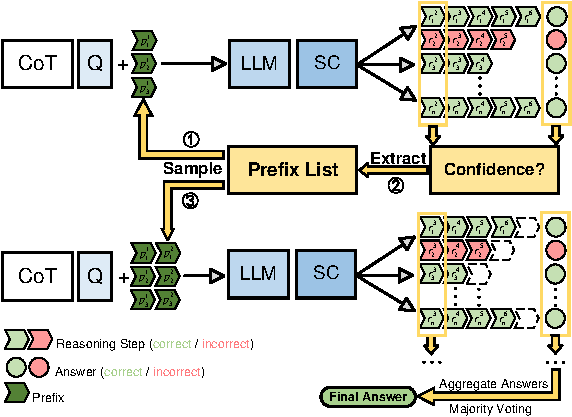
\includegraphics[width=0.75\linewidth]{figures/path-consistency-detail-v2.pdf}
\caption{An ``extract-and-sample'' inference process of the proposed path-consistency. It seeks the ``optimal path'' in the form of the ``prefix'', thereby progressively reducing the number of generated tokens and significantly shortening inference latency.}
\label{fig:path-consistency}
\vspace{-5mm}
\end{figure}

\section{Methodology}
\vspace{-2mm}
\subsection{Path-Consistency}\label{sec:path-consistency}
\vspace{-2mm}
% \begin{wrapfigure}{r}{0.5\textwidth}
% \centering
% 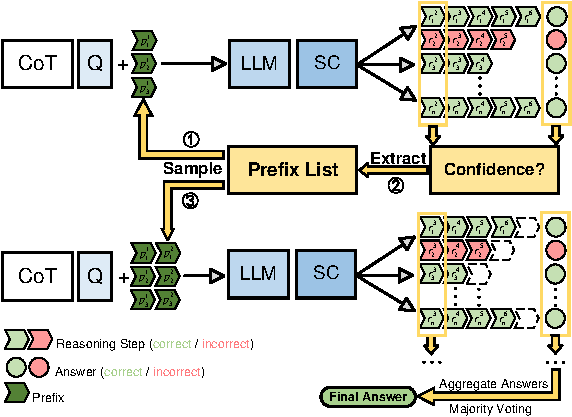
\includegraphics[trim=0cm 0cm 0cm 0cm, clip,height=5cm]{figures/path-consistency-detail-v2.pdf}
% \caption{An ``extract-and-sample'' inference process of the proposed path-consistency. It seeks the ``optimal path'' in the form of the ``prefix''. Thereby progressively reducing the number of generated tokens and significantly shortening inference latency.}
% \label{fig:path-consistency}
% \end{wrapfigure}

Based on the internal mechanisms of self-consistency, we propose an automated dynamic reasoning approach \textit{path-consistency} that continually seeks the ``optimal path'' in the form of ``prefix''. This will progressively reduce the number of generated tokens and significantly shorten inference latency. The methodology is shown in \cref{fig:path-consistency} and \cref{tab:path-consistency}, and can be described as the following ``extract-and-sample'' process:



\begin{itemize}[noitemsep, topsep=0pt, partopsep=0pt]
\item Determine the maximum number of branches and the highest prefix level for the specific task, and use these to divide all branches into multiple windows of equal length. Begin by generating a small number of branches for the first window. 
\item Then, use a confidence assessment metric\footnote{The proposed path-consistency allows a flexible choice of confidence assessment metrics (i.e., stopping criteria), based on intended objective and requirements. The confidence assessment metric used in the evaluation is the beta confidence criteria \cite{aggarwal2023let}.} to assess the confidence of the answers generated in the current window. If the confidence exceeds the set threshold, extract shorter prefixes from these optimal paths (e.g., the first step of the current optimal reasoning paths) to guide subsequent generation; if the confidence is low, continue generating branches for the subsequent windows at the current prefix level to ensure a safer prefix selection.
\item Randomly sample from the extracted prefixes as part of the prompt to guide subsequent generation. After the branches for the next window are generated, continue using the confidence assessment metric to find the optimal inference path and extract the prefix for the next level (e.g., the first two steps of the current optimal reasoning paths).
\item Repeat the above steps iteratively, extending the prefix length until the optimal reasoning path is identified and aggregated to produce the final answer.
\end{itemize}

\Cref{tab:path-consistency} illustrates the reasoning process of path-consistency with an example. We have taken a reasoning path from different stages of the branching process as samples in \cref{tab:path-consistency}. In the initial stage, the model generates the full reasoning paths and answers normally. When a particular answer appears frequently and has a higher confidence level compared to other answers within the current branch, the first step of the corresponding reasoning path is extracted and used as the input prompt for the next stage. As shown in \cref{tab:path-consistency}, as the number of branches increases, the prefix length grows while the newly generated portion of the path subsequently shortens.

\begin{table}[thp]
    % \vspace{-0.2cm}
    \setlength{\abovecaptionskip}{0.1cm}
    \caption{The generated parts are indicated in \color{blue}blue \color{black}in the table, with ``Level-$X$ prefix'' denoting the action of extracting the prefix for the $X^{th}$ time. After three prefix extractions, the model only needs to generate the final sentence of the conclusion based on the prefix.}
    \label{tab:path-consistency}
    \centering
    \small
    % \begin{tabular}{@{}l@{}}
    \begin{tabularx}{0.95\columnwidth}{@{}X@{}}
        \toprule
        
        \textbf{CoT-prompting:} \\
        Q: A robe takes 2 bolts of blue fiber and half that much white fiber. How many bolts in total does it take? \\
        A: \color{blue}{To make a robe, we need 2 bolts of blue fiber and half that much white fiber. We can write this as 2 + 1/2 * 2. Now 1/2 * 2 = 1, so the equation becomes 2 + 1 = 3. The answer is 3.} \\\\
        
        \textbf{Level-I prefix:} \\
        Q: A robe takes 2 bolts of blue fiber and half that much white fiber. How many bolts in total does it take? \\ 
        A: To make a robe, we need 2 bolts of blue fiber and half that much white fiber. \color{blue}{2 * 1/2 = 1 bolt of white fiber. 2 + 1 = 3 bolts in total. The answer is 3.} \\\\
        
        \textbf{Level-II prefix:} \\
        Q: A robe takes 2 bolts of blue fiber and half that much white fiber. How many bolts in total does it take? \\ 
        A: To make a robe, we need 2 bolts of blue fiber and half that much white fiber. 2 * 1/2 = 1 bolt of white fiber. \color{blue}{1 + 2 = 3 bolts in total. The answer is 3.} \\\\        
        \textbf{Level-III prefix:} \\
        Q: A robe takes 2 bolts of blue fiber and half that much white fiber. How many bolts in total does it take? \\ 
        A: To make a robe, we need 2 bolts of blue fiber and half that much white fiber. 2 * 1/2 = 1 bolt of white fiber. 1 + 2 = 3 bolts in total. \color{blue}{The answer is 3.} \\ \bottomrule
    \end{tabularx}
    % \end{tabular}
    % \vspace{-0.3cm}
\end{table}

When solving complex problems, LLM takes a question, represented as $q$, and generates a distribution of answers, denoted as $P(a\mid q)$, after producing a reasoning path. During inference, the model generates a multi-step reasoning path $ R = \left[ r^1, r^2, \cdots, r^T \right ] = r^{1:T}$  under the guidance of CoT. This process can also be expressed as 
% \vspace{-0.5cm}
\begin{equation}
    P(a\mid q)=\mathbb{E}_{R\sim P(R\mid q)}P(a\mid q,R).
\end{equation}
% \vspace{-0.5cm}

In basic self-consistency, the generation process is mechanically repeated numerous times without variation, whereas path-consistency attempts to gather advantageous intermediate information from the early stages of the generation process for subsequent generations. Path-consistency gradually identifies sufficiently confident partial reasoning steps $R_\text{prefix} = [r^1, r^2, \cdots, r^t]$ and incorporates them as part of the input, thereby better guiding the subsequent reasoning steps and the generation of the answer $a$. Thus, this process can be expressed as
% % \vspace{-0.5cm}
\begin{equation}
\small
    P(a\mid q, R_\text{prefix})=\mathbb{E}_{R\sim P(R\mid q, R_\text{prefix})}P(a\mid q, R).
\end{equation}
% \vspace{-0.5cm}

Combining the above expressions, we obtain the following formula via the law of total probability:
% \vspace{-0.5cm}
\begin{equation}
\small
    P(a\mid q)=\sum_{R_{\text{prefix}}}P(R_{\text{prefix}}\mid q)P(a\mid q, R_{\text{prefix}}).
\end{equation}
% \vspace{-0.5cm}
Path-consistency utilizes basic majority voting or other lightweight confidence metrics to model the distribution $P(R_{\text{prefix}}\mid q)$, facilitating the transformation from $P(a\mid q)$ to $P(a\mid q, R_\text{prefix})$. This approach enhances efficiency while maintaining the model's performance across various tasks.

\subsection{Reliability of Prefix Selection} \label{sec:reliability}

In the basic self-consistency method, when generating answers for particularly challenging questions, the problems with ``Truth Is in the Hands of a Few'' may still occur despite the repeated generation of multiple branches. This means that the correct answer may not be the most frequently occurring one, leading to an incorrect final answer in majority voting. In the proposed path-consistency method, during the continuous exploration for the optimal path, if the problems with ``Truth Is in the Hands of a Few'' are encountered at a specific prefix selection, there's a concern that this undesirable phenomenon may be exacerbated in subsequent branches. We will use the following to demonstrate that the proposed approach does not worsen this problem. 

To present the analysis, we make the following assumptions: the probability of generating the correct answer is $p_0$, and apart from the correct answer, the model generates only one unique incorrect answer. The total number of branches is set to $N$, and prefix selection based on majority voting is performed only once at $\frac{N}{2}$. % We use a single selection step purely to keep the exposition tractable; the actual algorithm applies the same beta-gated selection at every window boundary, and we validate the implications below empirically (prefix value curves and per-difficulty prefix survival rates in Section~\ref{sec:evaluation}).
If the correct answer is the majority at the time of prefix selection, the correct prefix will be selected to guide subsequent generation, increasing the probability of generating the correct answer in the remaining branches to $p_1 = p_0 + \Delta p$; Conversely, if the incorrect answer is the majority at this point, the probability of generating the correct answer in subsequent branches decreases to $p_2 = p_0 - \Delta p$. Using the binomial distribution formula, the probability of the correct answer being in the majority during the vote is given by:
\begin{equation}
    \small
    P_{\text{vote}}=\sum_{k=\lceil\frac{N}{4}\rceil}^{\frac{N}{2}}\binom{\frac{N}{2}}{k}p_0^k(1-p_0)^{\frac{N}{2}-k}.
\end{equation}

After prefix selection, the probability of obtaining the correct answer in the subsequent $\frac{N}{2}$ branches increases or decreases to
{
% scriptsize
\begin{scriptsize}
\begin{equation}
    \begin{aligned}\label{eq:p_inc}
        P_{\text{inc}} =&\sum_{k=\lceil\frac{N}{4}\rceil}^{\frac{N}{2}}\binom{\frac{N}{2}}{k}p_1^k(1-p_1)^{\frac{N}{2}-k} 
          = \sum_{k=\lceil\frac{N}{4}\rceil}^{\frac{N}{2}}\binom{\frac{N}{2}}{k}(p_0 + \Delta p)^k(1-p_0-\Delta p)^{\frac{N}{2}-k} \\
         = &\sum_{k=\lceil\frac{N}{4}\rceil}^{\frac{N}{2}}\binom{\frac{N}{2}}{k}p_0^k\left(1+\frac{\Delta p}{p_0}\right)^k(1-p_0)^{\frac{N}{2}-k}\left(1-\frac{\Delta p}{1-p_0}\right)^{\frac{N}{2} - k} \\
        \approx &  \sum_{k=\lceil\frac{N}{4}\rceil}^{\frac{N}{2}}\binom{\frac{N}{2}}{k}p_0^k(1-p_0)^{\frac{N}{2}-k}\left(1+\frac{k}{p_0}\Delta p\right)\left(1-\frac{\frac{N}{2}-k}{1-p_0}\Delta p\right) \\
        \approx & \sum_{k=\lceil\frac{N}{4}\rceil}^{\frac{N}{2}}\binom{\frac{N}{2}}{k}p_0^k(1-p_0)^{\frac{N}{2}-k}\left(1+\frac{k-\frac{N}{2}p_0}{p_0(1-p_0)}\Delta p\right),
\end{aligned}
\end{equation}
\end{scriptsize}
}
and
\begin{scriptsize}
\begin{equation}\label{eq:p_dec}
    % \small
    \begin{aligned}
        P_{\text{dec}}= & \sum_{k=\lceil\frac{N}{4}\rceil}^{\frac{N}{2}}\binom{\frac{N}{2}}{k}p_2^k(1-p_2)^{\frac{N}{2}-k}
        = \sum_{k=\lceil\frac{N}{4}\rceil}^{\frac{N}{2}}\binom{\frac{N}{2}}{k}(p_0 - \Delta p)^k(1-p_0 + \Delta p)^{\frac{N}{2}-k} \\
        \approx & \sum_{k=\lceil\frac{N}{4}\rceil}^{\frac{N}{2}}\binom{\frac{N}{2}}{k}p_0^k(1-p_0)^{\frac{N}{2}-k}\left(1-\frac{k-\frac{N}{2}p_0}{p_0(1-p_0)}\Delta p\right).
    \end{aligned}
\end{equation}
\end{scriptsize}

The two equations above use the first-order Taylor expansion, neglecting higher-order terms. The relationship between the two values is
\begin{equation} \label{eq:prove}
    P_{\text{inc}}+P_{\text{dec}}=2\cdot P_{\text{vote}}.
\end{equation}
Meanwhile, the final probability of obtaining the correct answer after prefix selection is
\begin{equation}
    P_\text{{correct}}^{\prime} = P_{\text{vote}}\cdot P_{\text{inc}} + (1 - P_{\text{vote}})\cdot P_{\text{dec}}.
\end{equation}

If no prefix selection is performed, the probability of generating the correct answer in subsequent steps remains unchanged and is equal to the probability at $\frac{N}{2}$ with majority voting: $P_\text{{correct}} =P_{\text{vote}}$.
% \begin{equation}
%     P_\text{{correct}} =P_{\text{vote}},
% \end{equation}
To ensure that accuracy is not adversely affected, we require $P_\text{{correct}}^{\prime}\geq P_{\text{correct}}$, which can be simplified to:
% \begin{equation}
%     P_\text{{correct}}^{\prime}\geq P_{\text{correct}},
% \end{equation}
% It can be simplified to:
\begin{equation}
    P_{\text{vote}}\geq \frac{P_{\text{vote}}-P_{\text{dec}}}{P_{\text{inc}}-P_{\text{dec}}}.
\end{equation}
By combining \cref{eq:prove}, we can obtain $P_{\text{vote}}\geq 0.5$. This proves that if the model's initial performance ensures $P_{\text{vote}}\geq 0.5$, path-consistency will be sufficiently reliable and will not harm accuracy.
% From this formula, we observe that the greater the difference between $P_{\text{inc}}$ and $P_{\text{dec}}$, the more reliable this method becomes, and the smaller the impact on accuracy.

During prefix selection, employing confidence-based criteria can make this process more reliable. For instance, using the beta confidence criteria \cite{aggarwal2023let}: let $n$ denote the number of branches generated so far and $v_m$ the number of votes received by the current majority answer. Under a uniform prior over the majority probability $\theta$ and a two-outcome (majority vs.\ rest) likelihood, the posterior is $\theta\mid n,v_m \sim \mathrm{Beta}(v_m+1,\, n-v_m+1)$, and the confidence that the majority answer is the correct one is
\begin{equation}\label{eq:confidence}
    \mathrm{conf}(n, v_m)
    = \Pr\!\Big(\theta \ge \tfrac{1}{2}\Bigm| n, v_m\Big)
    = \frac{\int_{1/2}^{1} p^{\,v_m}(1-p)^{\,n-v_m}\,dp}
           {\int_{0}^{1} p^{\,v_m}(1-p)^{\,n-v_m}\,dp}
    = 1 - I_{1/2}\big(v_m+1,\; n-v_m+1\big),
\end{equation}
where $I_{1/2}$ denotes the regularized incomplete beta function and $v_m$ represents the number of votes of the major element. A prefix is considered sufficiently reliable for selection only if this confidence exceeds a predefined threshold $C_{threshold}\in[0,1]$; setting $C_{threshold}=0$ turns the gate into plain majority-vote prefix selection, while $C_{threshold}=1$ recovers standard self-consistency (no prefix is ever promoted).

% If we roughly assume $N = 20$, $p_0=0.4$, $\Delta p = 0.01$, the final accuracy without prefix selection is $P_\text{{correct}} = 16.62\%$, and the final accuracy after prefix selection by majority voting is $P_\text{{voting}} = 15.15\%$, by Beta Stopping Criteria is $P_{C = 0.8} = 16.10\%$. Actually, $P_\text{{voting}} = P_{C = 0}$. Under the same conditions, if $p_0 = 0.6 (\ge 0.5)$, then both $P_{C = 0}$ and $P_{C = 0.8}$ will be greater than $P_\text{{correct}}$.

While this calculation is a rough estimate and the actual scenario is likely more complex, it provides insight into the reliability of prefix selection. Essentially, path-consistency tends to enhance the accuracy of self-consistency: when self-consistency performs well for a particular input, path-consistency may perform even better; when self-consistency performs poorly, the accuracy of path-consistency might decrease, but not significantly. Moreover, prefix selection guided by a confidence threshold provides a safer alternative to direct majority-vote selection. A more detailed analysis of beta-gated prefix promotion is provided in Appendix~\ref{app:promotion-soundness}, where we show that, under standard concentration assumptions, the probability of failing to promote a prefix with a positive correctness margin decays exponentially with the effective sample size.